% Options for packages loaded elsewhere
\PassOptionsToPackage{unicode}{hyperref}
\PassOptionsToPackage{hyphens}{url}
\documentclass[
  ignorenonframetext,
  aspectratio=169,
]{beamer}
\newif\ifbibliography
\usepackage{pgfpages}
\setbeamertemplate{caption}[numbered]
\setbeamertemplate{caption label separator}{: }
\setbeamercolor{caption name}{fg=normal text.fg}
\beamertemplatenavigationsymbolsempty
% remove section numbering
\setbeamertemplate{part page}{
  \centering
  \begin{beamercolorbox}[sep=16pt,center]{part title}
    \usebeamerfont{part title}\insertpart\par
  \end{beamercolorbox}
}
\setbeamertemplate{section page}{
  \centering
  \begin{beamercolorbox}[sep=12pt,center]{section title}
    \usebeamerfont{section title}\insertsection\par
  \end{beamercolorbox}
}
\setbeamertemplate{subsection page}{
  \centering
  \begin{beamercolorbox}[sep=8pt,center]{subsection title}
    \usebeamerfont{subsection title}\insertsubsection\par
  \end{beamercolorbox}
}
% Prevent slide breaks in the middle of a paragraph
\widowpenalties 1 10000
\raggedbottom
\AtBeginPart{
  \frame{\partpage}
}
\AtBeginSection{
  \ifbibliography
  \else
    \frame{\sectionpage}
  \fi
}
\AtBeginSubsection{
  \frame{\subsectionpage}
}
\usepackage{iftex}
\ifPDFTeX
  \usepackage[T1]{fontenc}
  \usepackage[utf8]{inputenc}
  \usepackage{textcomp} % provide euro and other symbols
\else % if luatex or xetex
  \usepackage{unicode-math} % this also loads fontspec
  \defaultfontfeatures{Scale=MatchLowercase}
  \defaultfontfeatures[\rmfamily]{Ligatures=TeX,Scale=1}
\fi
\usepackage{lmodern}
\ifPDFTeX\else
  % xetex/luatex font selection
\fi
% Use upquote if available, for straight quotes in verbatim environments
\IfFileExists{upquote.sty}{\usepackage{upquote}}{}
\IfFileExists{microtype.sty}{% use microtype if available
  \usepackage[]{microtype}
  \UseMicrotypeSet[protrusion]{basicmath} % disable protrusion for tt fonts
}{}
\makeatletter
\@ifundefined{KOMAClassName}{% if non-KOMA class
  \IfFileExists{parskip.sty}{%
    \usepackage{parskip}
  }{% else
    \setlength{\parindent}{0pt}
    \setlength{\parskip}{6pt plus 2pt minus 1pt}}
}{% if KOMA class
  \KOMAoptions{parskip=half}}
\makeatother
\usepackage{longtable,booktabs,array}
\usepackage{caption}
\captionsetup[table]{skip=6pt}
\newcounter{none} % for unnumbered tables
\usepackage{calc} % for calculating minipage widths
\usepackage{caption}
% Make caption package work with longtable
\makeatletter
\def\fnum@table{\tablename~\thetable}
\makeatother
\usepackage{graphicx}
\makeatletter
\newsavebox\pandoc@box
\newcommand*\pandocbounded[1]{% scales image to fit in text height/width
  \sbox\pandoc@box{#1}%
  \Gscale@div\@tempa{\textheight}{\dimexpr\ht\pandoc@box+\dp\pandoc@box\relax}%
  \Gscale@div\@tempb{\linewidth}{\wd\pandoc@box}%
  \ifdim\@tempb\p@<\@tempa\p@\let\@tempa\@tempb\fi% select the smaller of both
  \ifdim\@tempa\p@<\p@\scalebox{\@tempa}{\usebox\pandoc@box}%
  \else\usebox{\pandoc@box}%
  \fi%
}
% Set default figure placement to htbp
\def\fps@figure{htbp}
\makeatother
\setlength{\emergencystretch}{3em} % prevent overfull lines
\providecommand{\tightlist}{%
  \setlength{\itemsep}{0pt}\setlength{\parskip}{0pt}}
% Auto-generated by infrastructure/rendering/_pdf_latex_helpers.py::extract_math_font_preamble.
% Minimal header passed to Pandoc via -H so Beamer slides pick up the same math font
% as the combined-PDF path. Adjust the manuscript's preamble.md to change the font globally.
\usepackage{unicode-math}
\setmathfont{latinmodern-math.otf}

% Manuscript macro/package fallbacks (newcommand -> providecommand).
% Core mathematics
\usepackage{amsmath}
\usepackage{amssymb}
% Document layout
% Tables
\usepackage{booktabs}
% Caption styling (booktabs already loaded above). Small caption font with a
% bold label ("Figure 1", "Table 2") gives the math/figure-heavy layout a
% consistent, journal-like caption rhythm without fighting pandoc-crossref —
% pandoc emits standard \caption{}, and caption/captionsetup only restyle it.
% ── Theorem environments ─────────────────────────────────────────────────
% amsthm is loaded above. The FedGVI<->Friston bridge is stated as a small
% number of theorems/definitions/lemmas/propositions/corollaries; sharing one
% counter (definition/lemma/proposition/corollary all step the `theorem`
% counter) gives a single monotone numbering 1, 2, 3, ... across all kinds, so
% authors can reference them as Theorem 1, Definition 2, Corollary 3 without a
% per-kind counter drifting out of order. Plain style for theorem-like results,
% definition style (upright body) for definitions.
% (algorithm2e intentionally not loaded: this manuscript states results as
% numbered amsthm Theorems/Definitions, not algorithm2e pseudocode.)
% Code listings
\usepackage{listings}
% Typography and formatting
% (siunitx intentionally not loaded: no \SI/\num units appear in this manuscript.)
% Cross-references and citations
% (cleveref and titlesec intentionally not loaded: unavailable in this TeX tree
% and not required. Cross-references resolve through pandoc-crossref's own
% \ref-style names — no \cref appears — and section heading styling falls back
% to the pandoc/LaTeX defaults.)
% ── TeX Live Basic-compatible mono font for code listings ────────────
% Latin Modern Mono is bundled with TeX Live Basic and keeps the manuscript
% renderable on minimal TeX installations. Mathematical Unicode coverage is
% provided separately by Latin Modern Math below, so the code font does not
% need a private JuliaMono installation.
%
% Use the TeX font filename rather than the system-family name: the minimal
% TeX Live fontconfig database may not register the OpenType family even though
% kpsewhich can resolve the bundled files.
% Math font for unicode-math: Latin Modern Math (TeX Live) has full BMP
% coverage including U+2223 (\mid), U+226A/226B (\ll/\gg), and the Greek/
% blackboard letters used in equations. Without an explicit \setmathfont,
% unicode-math falls back to lmroman text font which lacks several glyphs
% and emits "Missing character" warnings on every \mid in math mode.

% Slide layout defaults for warning-clean scientific decks.
\usepackage{etoolbox}
\IfFileExists{xurl.sty}{\usepackage{xurl}}{}
\IfFileExists{seqsplit.sty}{\usepackage{seqsplit}}{\newcommand{\seqsplit}[1]{#1}}
\protected\def\breakseq#1{\seqsplit{#1}}
\protected\def\breaktt#1{\begingroup\ttfamily\seqsplit{#1}\endgroup}
\setlength{\emergencystretch}{6em}
\tolerance=5000
\hbadness=10000
\hfuzz=1pt
\setlength{\tabcolsep}{2pt}
\AtBeginEnvironment{longtable}{\tiny\renewcommand{\arraystretch}{0.86}\setlength{\tabcolsep}{1pt}}
\AtBeginEnvironment{tabular}{\tiny\renewcommand{\arraystretch}{0.86}\setlength{\tabcolsep}{1pt}}
\AtBeginEnvironment{equation}{\tiny}
\AtBeginEnvironment{equation*}{\tiny}
\AtBeginEnvironment{align}{\tiny}
\AtBeginEnvironment{align*}{\tiny}
\AtBeginEnvironment{itemize}{\footnotesize}
\AtBeginEnvironment{enumerate}{\footnotesize}
\AtBeginEnvironment{description}{\footnotesize}
\setbeamerfont{caption}{size=\tiny}
\setbeamerfont{caption name}{size=\tiny}
\setbeamerfont{normal text}{size=\small}
\setbeamerfont{frametitle}{size=\small}
\setbeamerfont{section title}{size=\footnotesize}
\setbeamerfont{subsection title}{size=\footnotesize}
\setbeamertemplate{section page}{%
  \centering
  \begin{beamercolorbox}[sep=12pt,center,wd=\paperwidth]{section title}
    \parbox{0.86\paperwidth}{\centering\usebeamerfont{section title}\insertsection\par}
  \end{beamercolorbox}
}
\setbeamertemplate{subsection page}{%
  \centering
  \begin{beamercolorbox}[sep=8pt,center,wd=\paperwidth]{subsection title}
    \parbox{0.86\paperwidth}{\centering\usebeamerfont{subsection title}\insertsubsection\par}
  \end{beamercolorbox}
}
\setlength{\abovecaptionskip}{2pt}
\setlength{\belowcaptionskip}{0pt}

% Natbib and cross-reference fallbacks — slides don't load natbib
% or cleveref, but combined-PDF manuscript prose may emit these
% commands. The fallback renders citations as a bracketed key list
% and cross-references as detokenized labels so slides don't fail on
% undefined control sequences or raw underscores. \providecommand is
% a no-op if packages load later.
\providecommand{\citep}[1]{[#1]}
\providecommand{\citet}[1]{#1}
\providecommand{\citealp}[1]{#1}
\providecommand{\citeauthor}[1]{#1}
\providecommand{\citeyear}[1]{#1}
\providecommand{\cref}[1]{\texttt{\detokenize{#1}}}
\providecommand{\Cref}[1]{\texttt{\detokenize{#1}}}
\providecommand{\crefrange}[2]{\texttt{\detokenize{#1}}--\texttt{\detokenize{#2}}}
\providecommand{\Crefrange}[2]{\texttt{\detokenize{#1}}--\texttt{\detokenize{#2}}}
\providecommand{\paragraph}[1]{\textbf{#1}\ }

% Opt-in accessible presentation profile.
\setbeamerfont{normal text}{size*={20pt}{24pt}}
\setbeamerfont{frametitle}{size*={28pt}{32pt}}
\setbeamerfont{section title}{size*={28pt}{32pt}}
\setbeamerfont{subsection title}{size*={28pt}{32pt}}
\setbeamerfont{caption}{size*={16pt}{19pt}}
\setbeamerfont{caption name}{size*={16pt}{19pt}}
\setbeamerfont{itemize/enumerate body}{size*={20pt}{24pt}}
\setbeamerfont{itemize/enumerate subbody}{size*={20pt}{24pt}}
\setbeamerfont{itemize/enumerate subsubbody}{size*={20pt}{24pt}}
\setbeamerfont{itemize item}{size*={20pt}{24pt}}
\setbeamerfont{itemize subitem}{size*={20pt}{24pt}}
\setbeamerfont{itemize subsubitem}{size*={20pt}{24pt}}
\setbeamerfont{description body}{size*={20pt}{24pt}}
\setbeamerfont{description item}{size*={20pt}{24pt}}
\setbeamerfont{quote}{size*={20pt}{24pt}}
\setbeamerfont{quotation}{size*={20pt}{24pt}}
\AtBeginEnvironment{longtable}{\fontsize{20pt}{24pt}\selectfont}
\AtBeginEnvironment{tabular}{\fontsize{20pt}{24pt}\selectfont}
\AtBeginEnvironment{equation}{\fontsize{20pt}{24pt}\selectfont}
\AtBeginEnvironment{equation*}{\fontsize{20pt}{24pt}\selectfont}
\AtBeginEnvironment{align}{\fontsize{20pt}{24pt}\selectfont}
\AtBeginEnvironment{align*}{\fontsize{20pt}{24pt}\selectfont}
\AtBeginEnvironment{itemize}{\fontsize{20pt}{24pt}\selectfont}
\AtBeginEnvironment{enumerate}{\fontsize{20pt}{24pt}\selectfont}
\AtBeginEnvironment{description}{\fontsize{20pt}{24pt}\selectfont}
\AtBeginDocument{\usebeamerfont{normal text}}
\newlength{\AFSlideTableWidth}
% The fixed footer reservation is calibrated with the semantic seven-line regular-body budget.
\setbeamertemplate{footline}{%
  \leavevmode\vbox{%
    \hbox{%
      \begin{beamercolorbox}[wd=\paperwidth,ht=16pt,dp=3pt,center]{author in head/foot}%
        \fontsize{16pt}{19pt}\selectfont Untagged PDF derivative \textbar\ \href{../web/index.html}{HTML reader}%
      \end{beamercolorbox}%
    }%
    \vskip6pt%
  }%
}
% Accessible footer reserved height: 25pt.

\newtheorem{proposition}{Proposition}
\newtheorem{hypothesis}{Hypothesis}
\newtheorem{remark}[theorem]{Remark}
\newtheorem{axiom}{Axiom}
\newtheorem{property}{Property}
\usepackage{bookmark}
\IfFileExists{xurl.sty}{\usepackage{xurl}}{} % add URL line breaks if available
\urlstyle{same}
% fallback for those not using the hyperref driver hyperxmp:
\makeatletter
\@ifundefined{xmpquote}{\newcommand{\xmpquote}[1]{#1}}{}
\makeatother
\hypersetup{
  hidelinks,
  pdfcreator={LaTeX via pandoc}}

\author{\texorpdfstring{}{}}
\date{}

\begin{document}

\section{Supplement: variational aggregation objective and weight
control}\label{sec:supp-variational}

\begin{frame}[fragile]{Supplement: variational aggregation objective and
weight control}
\ifcsname proposition\endcsname
\else
\newtheorem{proposition}{Proposition}
\fi

This supplement gives the full derivation behind
sec.~5.8.2: the server-side aggregator
\texttt{robust\_aggregate} is a heuristic,
\end{frame}

\begin{frame}{Supplement: variational\ldots{} (part 2)}
and a single change of divergence direction turns it into
block-coordinate descent on a stated free energy with a derived,
redescending effective-weight update.
\end{frame}

\begin{frame}{Supplement: variational\ldots{} (part 3)}
We work throughout with categorical local posteriors \(q_n(s)\) over the
shared latent factor, base weights \(w_n > 0\), robustness \(c > 0\),
and the consensus \(q\) on the probability simplex. Let \(\lambda>0\) be
the entropy-weight coefficient, with the current default at
\(\lambda=1.0\).
\end{frame}

\begin{frame}{Why the sharp heuristic is not yet variational}
\protect\phantomsection\label{sec:supp-why-heuristic}
The sharp server rule is empirically strong, but this repository has not
established a variational certificate for it.
\end{frame}

\begin{frame}{Why the sharp heuristic is\ldots{} (part 2)}
The heuristic of eq.~10 alternates a
\emph{reverse-KL} weight update
\(a_n \leftarrow w_n\exp(-c\,\mathrm{KL}(q_n \,\|\, q))\).
\end{frame}

\begin{frame}{Why the sharp heuristic is\ldots{} (part 3)}
It couples that update with the log-linear consensus
\(q \leftarrow \mathrm{softmax}(\sum_n a_n \log q_n)\). For the natural
direct objective \(\sum_n a_n \mathrm{KL}(q_n \,\|\, q) +
\tfrac{1}{c}\mathrm{KL_{gen}}(a\,\|\,w)\), the reverse-KL rule is the
\(a\)-minimizer.
\end{frame}

\begin{frame}{Why the sharp heuristic is\ldots{} (part 4)}
The \(q\)-minimizer is the \emph{arithmetic} (linear) pool
\(q \propto \sum_n a_n q_n\), not the log-linear pool. The executable
orientation witness confirms this finite-simplex mismatch. The following
proposition goes further, while retaining a deliberately narrow scope.
\end{frame}

\begin{frame}{Why the sharp heuristic is\ldots{} (part 5)}
\begin{equation}\tag{24}\protect\phantomsection\label{eq:raw-log-pool-block}{
Q(a;s) \;=\; \operatorname{softmax}\!\left(\sum_n a_n\log s_n\right)
}\end{equation}
\end{frame}

\begin{frame}{Why the sharp heuristic is\ldots{} (part 6)}
The proposed raw \(q\)-block is the map in
eq.~24.
\end{frame}

\begin{frame}{Why the sharp heuristic is\ldots{} (part 7)}
\begin{equation}\tag{25}\protect\phantomsection\label{eq:separable-server-objective}{
\begin{aligned}
F(q,a;s,w)
&= \sum_n a_n\,\mathrm{KL}(q\,\|\,s_n)\\
&\quad + R(a,w) + G(q).
\end{aligned}
}\end{equation}
\end{frame}

\begin{frame}{Why the sharp heuristic is\ldots{} (part 8)}
\begin{proposition}[Scoped separable raw-log-pool no-go]\label{prop:raw-log-pool-no-go}
For \(K\geq2\), no objective in (25) satisfying
the declared separability and differentiability conditions has \(Q(a;s)\) as
its \(q\)-coordinate minimizer for every positive interior \(a\) and \(s\).
\end{proposition}
\end{frame}

\begin{frame}{Why the sharp heuristic is\ldots{} (part 9)}
Precisely, \(G\) is continuously differentiable and independent of
\(a,s\), while \(R\) is independent of \(q,s\). Under those conditions,
this objective class cannot realize both block maps of the implemented
raw-weight heuristic.
\end{frame}

\begin{frame}{Why the sharp heuristic is\ldots{} (part 10)}
\emph{Proof sketch.} Fix any non-uniform interior \(q\), a positive
scalar \(\alpha\), and one local posterior constructed in
eq.~26:
\end{frame}

\begin{frame}{Why the sharp heuristic is\ldots{} (part 11)}
\begin{equation}\tag{26}\protect\phantomsection\label{eq:raw-log-pool-witness-source}{
s_i^{(\alpha)} \;=\;
\frac{q_i^{1/\alpha}}{\sum_j q_j^{1/\alpha}}.
}\end{equation}
\end{frame}

\begin{frame}{Why the sharp heuristic is\ldots{} (part 12)}
Then \(Q(\alpha;s^{(\alpha)})=q\). Writing \(\Pi\) for projection onto
the tangent space of the simplex, first-order stationarity of
eq.~25 at that same \(q\) requires
\(\Pi[(\alpha-1)\log q+\nabla G(q)]=0\).
\end{frame}

\begin{frame}{Why the sharp heuristic is\ldots{} (part 13)}
The unit-scale construction forces \(\Pi\nabla G(q)=0\); any different
positive scale then forces \(\Pi\log q=0\), contradicting the
non-uniform choice of \(q\). The executable witness records both exact
log-pool identities and the nonzero tangential contradiction.
\end{frame}

\begin{frame}{Why the sharp heuristic is\ldots{} (part 14)}
A companion witness also blocks the obvious normalized-weight escape
within the same natural data-term class: two interior consensuses yield
the same normalized reverse-KL weights but different forward-KL
data-term differences,
\end{frame}

\begin{frame}{Why the sharp heuristic is\ldots{} (part 15)}
so a \(q\)-independent differentiable \(R(a,w)\) cannot satisfy both
simplex-stationarity equations. The implementation itself uses raw
effective weights, so this companion is a scope check rather than a
description of the production update.
\end{frame}

\begin{frame}[fragile]{Why the sharp heuristic is\ldots{} (part 16)}
% template-accessible-table-inset
\begingroup
\setlength{\AFSlideTableWidth}{\textwidth}%
\setlength{\LTleft}{\fill}%
\setlength{\LTright}{\fill}%
\begin{longtable}[]{@{}
  >{\raggedright\arraybackslash}p{(\AFSlideTableWidth - 2\tabcolsep) * \real{0.3529}}
  >{\raggedright\arraybackslash}p{(\AFSlideTableWidth - 2\tabcolsep) * \real{0.6471}}@{}}
\label{tbl:server-theory-witness}\tabularnewline
\toprule\noalign{}
\begin{minipage}[b]{\linewidth}\raggedright
Artifact
\end{minipage} & \begin{minipage}[b]{\linewidth}\raggedright
Implementation surface and declared scope
\end{minipage} \\
\midrule\noalign{}
\endfirsthead
\toprule\noalign{}
\begin{minipage}[b]{\linewidth}\raggedright
Artifact
\end{minipage} & \begin{minipage}[b]{\linewidth}\raggedright
Implementation surface and declared scope
\end{minipage} \\
\midrule\noalign{}
\endhead
Raw contradiction & \texttt{server\_theory.py}; interior inputs and raw
\(q\)-block \\
\bottomrule\noalign{}
\end{longtable}
\endgroup
\end{frame}

\begin{frame}{Why the sharp heuristic is\ldots{} (part 17)}
The witness table in tbl.~13 records the
deterministic implementation surfaces that bind this scoped result to
the typed analysis report.
\end{frame}

\begin{frame}{Why the sharp heuristic is\ldots{} (part 18)}
The proposition does \textbf{not} say that no objective of any kind
exists. It does not exclude nonseparable \(q\)--\(a\) couplings,
source-dependent terms, non-differentiable constructions, or objectives
that encode selected fixed points without reproducing the update blocks
for all interior inputs.
\end{frame}

\begin{frame}{Why the sharp heuristic is\ldots{} (part 19)}
Thus sec.~5.8 retains the heuristic label and
claims only the recovery limit, the scoped negative result above, and
conditional empirical behavior --- never a bounded-influence property or
an objective-backed status.
\end{frame}

\begin{frame}{Aggregation free energy and its block minimizers}
\protect\phantomsection\label{sec:supp-derivation}
\begin{definition}[Aggregation free energy]\label{def:aggregation-free-energy}
For \(c,\lambda>0\), consensus \(q\), and nonnegative effective weights
\(a=(a_n)\), define \(F_\lambda(q,a)\) by (12), where
\(\mathrm{CE}(q,q_n)=-\sum_i q_i\log q_{n,i}\), \(H(q)\) is entropy, and
\(\mathrm{KL}_{\rm gen}(a\|w)=\sum_n g_n\) for
\(g_n=a_n\log(a_n/w_n)-a_n+w_n\).
\end{definition}
\end{frame}

\begin{frame}{Aggregation free energy\ldots{} (part 2)}
\textbf{The \(q\)-block.} For \(\lambda>0\), fixing \(a\), the
\(q\)-dependent part of \(F_\lambda\) is denoted \(J(q;a)\) and can be
written in either of two equivalent forms:
\end{frame}

\begin{frame}{Aggregation free energy\ldots{} (part 3)}
\begin{equation}\tag{27}\protect\phantomsection\label{eq:agg-q-objective}{
\begin{aligned}
J(q;a)
&=\sum_n a_n\,\mathrm{CE}(q,q_n)-\lambda H(q),\\
J(q;a)
&=\lambda\sum_i q_i\log q_i\\
&\quad-\sum_i\sum_n q_i a_n\log q_{n,i}.
\end{aligned}
}\end{equation}
\end{frame}

\begin{frame}{Aggregation free energy\ldots{} (part 4)}
Adding a Lagrange multiplier to the block in
eq.~27 for \(\sum_i q_i = 1\) and differentiating
gives \(\lambda\log q_i + \lambda - \sum_n a_n \log q_{n,i} + \mu = 0\),
i.e.
\end{frame}

\begin{frame}{Aggregation free energy\ldots{} (part 5)}
\begin{equation}\tag{28}\protect\phantomsection\label{eq:agg-q-min}{
\begin{aligned}
q_i
&\propto \exp\!\Big(
  \tfrac{1}{\lambda}\sum_n a_n \log q_{n,i}\Big),\\
q_i
&= \mathrm{softmax}\!\Big(
  \tfrac{1}{\lambda}\sum_n a_n \log q_n\Big)_i.
\end{aligned}
}\end{equation}
\end{frame}

\begin{frame}{Aggregation free energy\ldots{} (part 6)}
the product of the weighted experts --- the consensus update of
eq.~13. At the default \(\lambda=1.0\), the \(-H(q)\)
term sharpens the weighted geometric mean into the product-of-experts
(the entropy bonus that makes the project's log-linear pool a product
rather than a geometric average).
\end{frame}

\begin{frame}{Aggregation free energy\ldots{} (part 7)}
\textbf{The \(a\)-block.} Fixing \(q\),
\(\partial F/\partial a_n = \mathrm{CE}(q,q_n) + \tfrac{1}{c}\log(a_n/w_n) = 0\),
so
\end{frame}

\begin{frame}{Aggregation free energy\ldots{} (part 8)}
\begin{equation}\tag{29}\protect\phantomsection\label{eq:agg-a-min}{
a_n \;=\; w_n\,\exp\!\big(-c\,\mathrm{CE}(q, q_n)\big),
}\end{equation}
\end{frame}

\begin{frame}{Aggregation free energy\ldots{} (part 9)}
the weight update of eq.~13. Because
\(\mathrm{CE}(q,q_n) = H(q) + \mathrm{KL}(q\,\|\,q_n)\), the forward
direction \(\mathrm{KL}(q\,\|\,q_n)\) --- not the heuristic's reverse
\(\mathrm{KL}(q_n\,\|\,q)\) --- is the one consistent with the consensus
update.
\end{frame}

\begin{frame}{Aggregation free energy\ldots{} (part 10)}
Each block update is the \emph{exact} minimizer of its block, so
alternating them is block-coordinate descent: \(F\) is non-increasing at
every half-step. When the iterates converge, their fixed point is
coordinatewise stationary.
\end{frame}

\begin{frame}{Aggregation free energy\ldots{} (part 11)}
The implementation keeps numerical failure handling outside that
theorem. If finite-precision underflow collapses all effective weights,
it records a fallback event, substitutes the declared base weights to
return a valid probability vector, and does not certify the substituted
trajectory as converged.
\end{frame}

\begin{frame}{Aggregation free energy\ldots{} (part 12)}
Such a trace is diagnostic evidence about the solver boundary, not an
instance of the exact block-descent result.
\end{frame}

\begin{frame}{Conservative-server properties}
\protect\phantomsection\label{sec:supp-theorem}
\begin{theorem}[Properties]
\label{thm:variational-aggregation}
For \(c,\lambda>0\), (28)–(29) make \(F\)
non-increasing. At convergence, \((q^*,a^*)\) is coordinatewise stationary.
As \(c\to0\), \(a_n\to w_n\) and \(q\) tends to the tempered log-linear pool;
\(\lambda=1.0\) gives
(9). Finally,
\(a_n=w_n\exp[-c\,\mathrm{CE}(q,q_n)]\le w_n\), and
\(\mathrm{KL}(q\,\|\,q_n)\to\infty\) gives \(a_n\to0\).
\end{theorem}
\end{frame}

\begin{frame}{Conservative-server\ldots{} (part 2)}
The variational aggregator therefore shares the project log-linear-pool
corner of (10). Under the qualified bridge of
sec.~5.8, this is only the categorical
message-combination specialization, not the complete source protocol.
\end{frame}

\begin{frame}{Conservative-server\ldots{} (part 3)}
The final inequality makes the raw effective-weight update bounded and
redescending relative to the realized consensus. It does not by itself
establish a bounded influence function or finite gross-error sensitivity
for the normalized consensus estimator.
\end{frame}

\begin{frame}{Conservative-server\ldots{} (part 4)}
The objective \(F\) is biconvex (each block convex, the coupling
\(\sum_n a_n\mathrm{CE}(q,q_n)\) bilinear), so the result concerns
monotone block updates and converged coordinatewise fixed points, not
guaranteed convergence to or certification of a global minimum.
\end{frame}

\begin{frame}{Conservative-server\ldots{} (part 5)}
\textbf{The effective-weight regime, and why multi-start matters.} The
weight bound \(a_n \le w_n\) is unconditional
(\(\mathrm{CE}(q,q_n)\ge 0\) always). The \emph{collapse} \(a_n \to 0\)
is driven by the agent's divergence \emph{from the realized consensus}
\(\mathrm{KL}(q\,\|\,q_n)\), and the consensus itself depends on the
weights.
\end{frame}

\begin{frame}{Conservative-server\ldots{} (part 6)}
Because \(F\) is biconvex, this couples into a subtlety an adversarial
review of this work surfaced: a \emph{near-one-hot} saboteur
(contamination rate \(\to 1\)) already captures the product-of-experts,
so a descent seeded \emph{at} that pool stays in a consensus-capture
basin (high \(F\)) where the saboteur keeps its weight ---
\end{frame}

\begin{frame}{Conservative-server\ldots{} (part 7)}
even against an honest majority.
\end{frame}

\begin{frame}[fragile]{Conservative-server\ldots{} (part 8)}
The repair is to search the stated objective more carefully:
\texttt{variational\_aggregate} runs \textbf{multi-start}
block-coordinate descent (the pool, the uniform belief, and the
arithmetic-mean seeds) and returns the lowest-observed-\(F\) converged
candidate.
\end{frame}

\begin{frame}{Conservative-server\ldots{} (part 9)}
In the configured colony, the uniform/arithmetic seeds reach a
lower-\(F\) \emph{vetoing} basin, so the saboteur is suppressed even at
the simplex vertex (pinned qualitatively by the near-vertex multi-start
test) --- the 267.1\(\times\) suppression of
fig.~17 is measured across the swept
contamination grid,
\end{frame}

\begin{frame}{Conservative-server\ldots{} (part 10)}
whose most extreme point sits just below rate \(1\).
\end{frame}

\begin{frame}{Conservative-server\ldots{} (part 11)}
What remains fundamental to \emph{every} robust fusion rule, and is not
claimed away: with no honest majority --- a colony split with no
anchoring plurality --- there is no truth to recover.
\end{frame}

\begin{frame}{Conservative-server\ldots{} (part 12)}
The observed suppression is conditional on the tested colonies and the
fixed point selected by a finite multi-start heuristic.
\end{frame}

\begin{frame}{Conservative-server\ldots{} (part 13)}
fig.~21 makes the capture and the escape
concrete on a near-vertex colony: the single (log-linear-pool) start
settles at \(F = 1.3092\) (the higher observed basin, where the saboteur
keeps its weight), while one of the configured alternative starts
reaches a lower observed basin at \(F = -0.2305\) ---
\end{frame}

\begin{frame}{Conservative-server\ldots{} (part 14)}
a gap of 1.5397 nats. This finite multistart comparison shows that the
natural seed can be captured; it neither exhausts all basins nor
certifies a global optimum.
\end{frame}

\begin{frame}{Conservative-server\ldots{} (part 15)}
\begin{figure}
\centering
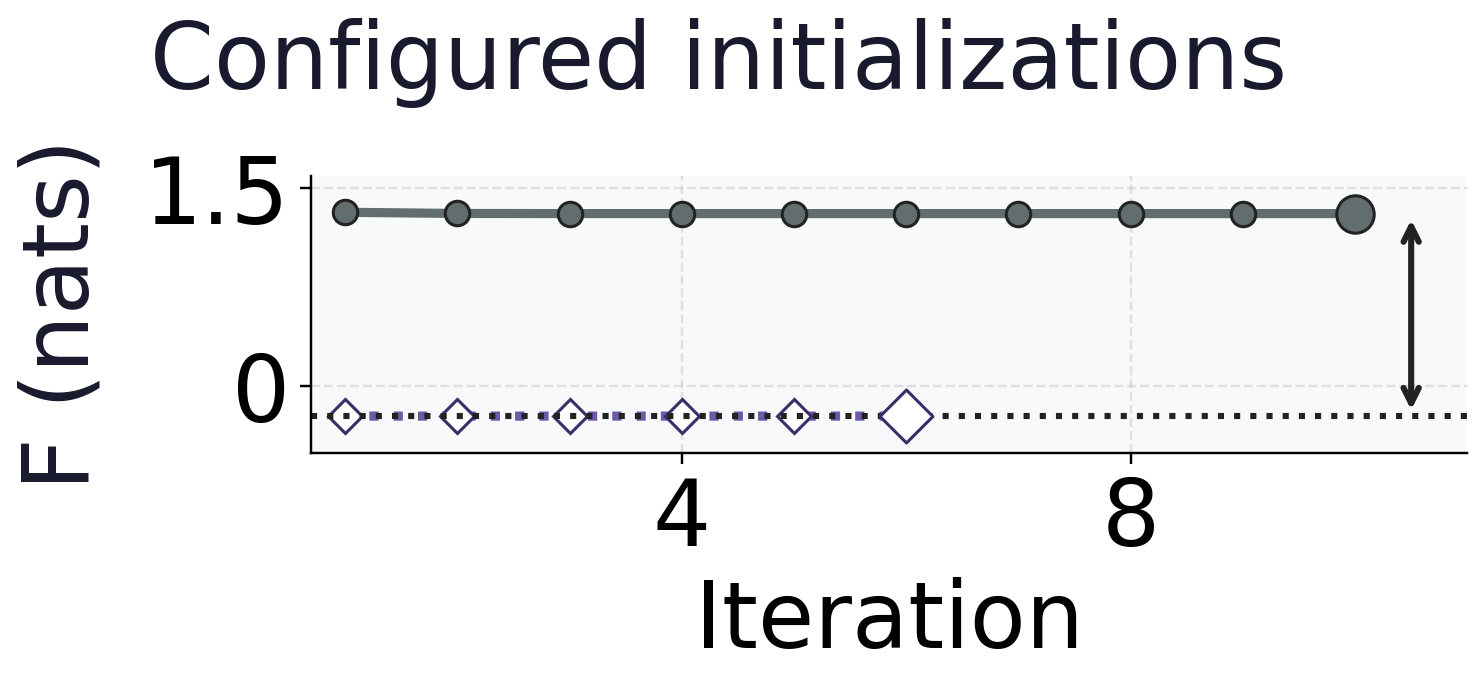
\includegraphics[keepaspectratio,width=0.98\linewidth,height=0.8\textheight,alt={Both complete objective trajectories, observed endpoints, lower final reference and terminal gap.}]{../figures/descent_comparison.slide-trajectories.png}
\refstepcounter{figure}\label{fig:descent-comparison-slide-panel-1}
\end{figure}
\end{frame}

\begin{frame}{Conservative-server\ldots{} (part 16)}
\begin{figure}
\centering
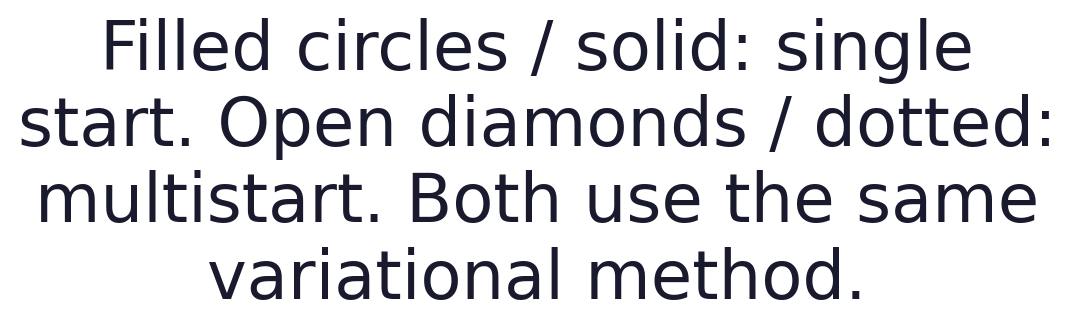
\includegraphics[keepaspectratio,width=0.98\linewidth,height=0.8\textheight,alt={Filled circles / solid: single start. Open diamonds / dotted: multistart. Both use the same variational method.}]{../figures/descent_comparison.slide-key.png}
\refstepcounter{figure}\label{fig:descent-comparison-slide-panel-2}
\end{figure}
\end{frame}

\begin{frame}{Conservative-server\ldots{} (part 17)}
\begin{figure}
\centering
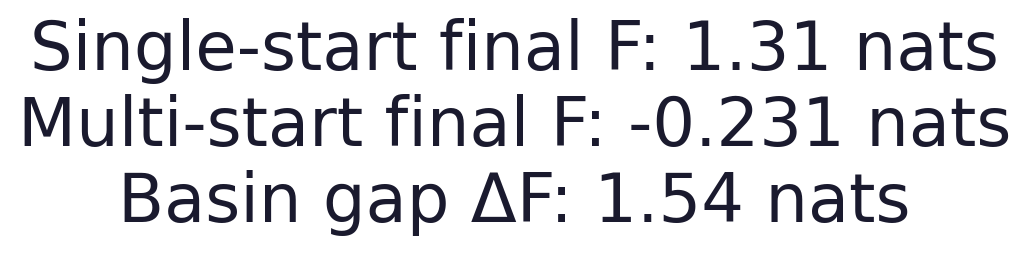
\includegraphics[keepaspectratio,width=0.98\linewidth,height=0.8\textheight,alt={Single-start final F: 1.31 nats
Multi-start final F: -0.231 nats
Basin gap ΔF: 1.54 nats}]{../figures/descent_comparison.slide-notes-1.png}
\refstepcounter{figure}\label{fig:descent-comparison-slide-panel-3}
\end{figure}
\end{frame}

\begin{frame}{Conservative-server\ldots{} (part 18)}
\begin{figure}
\centering
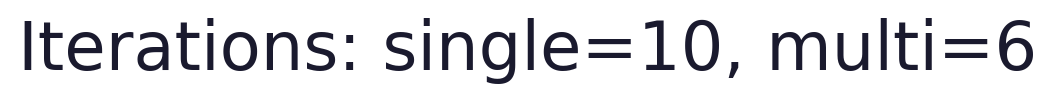
\includegraphics[keepaspectratio,width=0.98\linewidth,height=0.8\textheight,alt={Iterations: single=10, multi=6}]{../figures/descent_comparison.slide-notes-2.png}
\refstepcounter{figure}\label{fig:descent-comparison-slide-panel-4}
\end{figure}
\end{frame}

\begin{frame}{Conservative-server\ldots{} (part 19)}
\begin{figure}
\centering
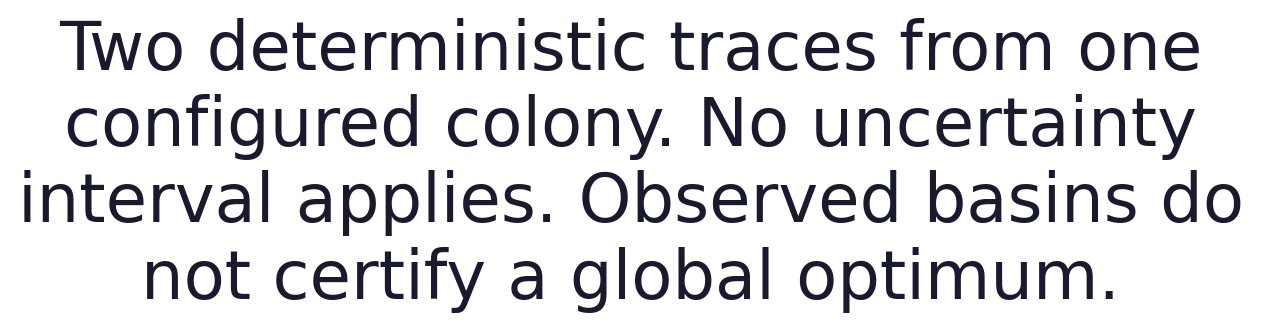
\includegraphics[keepaspectratio,width=0.98\linewidth,height=0.8\textheight,alt={Two deterministic traces from one configured colony. No uncertainty interval applies. Observed basins do not certify a global optimum.}]{../figures/descent_comparison.slide-scope.png}
\refstepcounter{figure}\label{fig:descent-comparison-slide-panel-5}
\end{figure}
\end{frame}

\begin{frame}[fragile]{Numerical witnesses for descent and influence
bounds}
\protect\phantomsection\label{sec:supp-witnesses}
The analysis pipeline runs \texttt{variational\_aggregate} at robustness
\(c = 1.50\) on a contaminated colony and records the free energy after
each iteration.
\end{frame}

\begin{frame}{Numerical witnesses for\ldots{} (part 2)}
The descent falls from \(F = 3.2458\) to \(F = 2.3780\) (a monotone drop
of \(0.8678\) over 11 iterations, converged: Yes); the largest
single-step \emph{increase} is \(8.88 \times 10^{-16}\), machine zero
--- the monotonicity of the theorem,
\end{frame}

\begin{frame}{Numerical witnesses for\ldots{} (part 3)}
witnessed numerically and drawn in fig.~16.
\end{frame}

\begin{frame}{Numerical witnesses for\ldots{} (part 4)}
For the effective-weight diagnostic, one agent is drifted from healthy
toward a confident-wrong delta and its normalized influence is read at
each drift. Clean, it carries \(0.143\) of the pool; at the most extreme
swept drift it carries below \(0.001\) --- a factor of 267.1 (computed
from the unrounded influences,
\end{frame}

\begin{frame}{Numerical witnesses for\ldots{} (part 5)}
not the display-rounded values above) below the fixed 0.143 the naive
pool would still grant it (fig.~17).

This makes the redescending normalized-weight behavior visible on the
tested path; it is not an estimator-level B-robustness proof.
\end{frame}

\begin{frame}{Tempered aggregation family for the accuracy-guarantee
trade}
\protect\phantomsection\label{sec:supp-tempered}
The aggregator of sec.~12.2 fixes the entropy term
at unit weight. Relaxing that single coefficient generates a
one-parameter \emph{tempered} family. Introduce an entropy weight
\(\lambda > 0\) ---
\end{frame}

\begin{frame}{Tempered aggregation\ldots{} (part 2)}
the \textbf{inverse temperature is} \(1/\lambda\) --- and minimize
\end{frame}

\begin{frame}{Tempered aggregation\ldots{} (part 3)}
\begin{equation}\tag{30}\protect\phantomsection\label{eq:tempered-family}{
\begin{aligned}
F_\lambda(q, a)
&= \sum_n a_n\,\mathrm{CE}(q, q_n) - \lambda H(q)\\
&\quad + \tfrac{1}{c}\,\mathrm{KL_{gen}}(a \,\|\, w).
\end{aligned}
}\end{equation}
\end{frame}

\begin{frame}{Tempered aggregation\ldots{} (part 4)}
Repeating the \(q\)-block derivation of eq.~28 with the
entropy scaled by \(\lambda\) leaves the \(a\)-block \textbf{untouched}
and tempers only the consensus update:
\end{frame}

\begin{frame}{Tempered aggregation\ldots{} (part 5)}
\begin{equation}\tag{31}\protect\phantomsection\label{eq:tempered-updates}{
\begin{aligned}
q
&\propto \exp\!\Big(
  \tfrac{1}{\lambda}\textstyle\sum_n a_n \log q_n\Big),\\
a_n
&= w_n\,\exp\!\big(-c\,\mathrm{CE}(q, q_n)\big).
\end{aligned}
}\end{equation}
\end{frame}

\begin{frame}{Tempered aggregation\ldots{} (part 6)}
The \(\lambda\downarrow0\) endpoint is separately implemented as a
deterministic tied-argmax rule; it is not obtained by substituting
\(\lambda=0\) into eq.~30 or
eq.~31.
\end{frame}

\begin{frame}{Tempered aggregation\ldots{} (part 7)}
The weight update is \textbf{independent of \(\lambda\)}: the bound
\(a_n \le w_n\) with collapse \(a_n \to 0\) as
\(\mathrm{KL}(q\,\|\,q_n) \to \infty\) is unchanged, so the \textbf{raw
effective-weight bound of sec.~12.3 holds for every}
\(\lambda > 0\).
\end{frame}

\begin{frame}{Tempered aggregation\ldots{} (part 8)}
At \(\lambda = 1.0\) the temperature is unity and
eq.~31 is \textbf{identical} to the current
axis-3 aggregator eq.~13 --- the default is
bit-identical, not merely close.
\end{frame}

\begin{frame}{Tempered aggregation\ldots{} (part 9)}
The \(c \to 0\) recovery of sec.~12.3 generalizes to
the \emph{tempered} log-linear pool
\(q \propto \exp(\tfrac{1}{\lambda}\sum_n w_n \log q_n)\); at
\(\lambda = 1.0\) this is exactly
\(\mathrm{softmax}(\sum_n w_n \log q_n)\) --- the project's
\textbf{log-linear pool} eq.~9.
\end{frame}

\begin{frame}{Tempered aggregation\ldots{} (part 10)}
Under the shared-support, posterior-log-potential, and fixed-weight
assumptions of sec.~5.8, that pool is a
categorical specialization of Friston Eq. 7's message-combination term,
not a reconstruction of the complete source protocol.
\end{frame}

\begin{frame}{Tempered aggregation\ldots{} (part 11)}
Positive-temperature members away from that default are tempered pools,
not Friston Eq. 7 itself; the project recovery checks, including ISC-10,
remain project-local.
\end{frame}

\begin{frame}{Tempered aggregation\ldots{} (part 12)}
A small empirical sweep over
\(\lambda \in \{ 0.1, 0.2, 0.3, 0.5, 0.7, 1 \}\) on 10 contaminated
colonies (5 agents, 2 adversarial) asks whether a single
\(\lambda^{\ast}\) makes the conservative aggregator narrow the gap to
the sharp \(\mathrm{robust\_aggregate}\) point-accuracy.
\end{frame}

\begin{frame}{Tempered aggregation\ldots{} (part 13)}
The closest observed weight is \(\lambda^{\ast} = 0.3\) with an accuracy
gap of 0.0008. \textbf{A lambda* narrows the tested accuracy gap while
preserving the stated weight bound on this grid.} If no \(\lambda\)
closes that gap while preserving the derived weight update, the result
is the conservatism trade-off of sec.~8.13,
\end{frame}

\begin{frame}{Tempered aggregation\ldots{} (part 14)}
not a defect to hide.
\end{frame}

\end{document}
